%
%  Chad Conrad
%
\documentclass[12pt,fullpage]{article}
\usepackage{fullpage}
\usepackage{amsmath}
\usepackage{psfrag}                                          % LaTeX graphics tool
\usepackage{pslatex}                                         % avoids the default cmr font
\usepackage{graphicx}                                        % graphics package 
\usepackage{epsfig}                                          % figures
\usepackage{hyperref}
\usepackage{color}

\begin{document}

\noindent
{\bf Discrete uniform distribution} (from \color{blue}\url{http://www.math.wm.edu/~leemis/chart/UDR/UDR.html}\color{black})

\noindent
The shorthand $X \sim \textrm{discrete uniform}(a,b)$ is used to indicate that the
random variable $X$ has the discrete uniform distribution with integer parameters $a$ and $b$, where  $a<b$.
A discrete uniform random variable $X$ with parameters $a$ and $b$ has probability mass function 
$$
f(x) = \frac{1}{b-a+1} \qquad \qquad x=a, \kern 0.08 em a+1, \ldots, b.
$$
The probability mass function is illustrated below.
{\begin{figure}[h!]
\begin{center}
\psfrag{laba}{$a$}
\psfrag{labb}{$b$}
\psfrag{labx}{$x$}
\psfrag{labf}{$f(x)$}
\psfrag{labff}{$\frac{1}{b-a+1}$}
\psfrag{lab1}{$\cdots$}
\psfrag{lab2}{$\cdots$}
\includegraphics[width=3.2in]{DiscreteuniformPlot.ps}
\end{center}
\end{figure}}\\
The cumulative distribution function is
$$
F(x) = P(X \le x) = \frac{x-a+1}{b-a+1} \qquad \qquad x=a, \kern 0.08 em a+1, \ldots ,b.\\
$$
The survivor function of $X$ is
$$
S(x) = P(X \ge x) = \frac{b-x+1}{b-a+1} \qquad \qquad x=a, \kern 0.08 em a+1, \ldots ,b.\\
$$
The hazard function of $X$ is
$$
h(x) = \frac{f(x)}{S(x)} = \frac{1}{b-x+1} \qquad \qquad x=a,\kern 0.08 em  a+1, \ldots ,b.\\
$$
The inverse distribution function of $X$ is
$$
F ^ {-1}(u) = a+ \left\lfloor u(b-a+1) \right\rfloor \qquad \qquad 0 < u < 1.
$$
The median, $m$, of $X$ is
$$
m = \frac{a+b}{2}.
$$
The moment generating function of $X$ is
$$
M(t) = E\left[ e ^ {tX} \right] = \frac{e^{at}-e^{(b+1)t}}{(b-a+1)(1-e^{t})} \qquad \qquad -\infty < t < \infty.
$$
The characteristic function of $X$ is
$$
\phi(t) = E\left[ e ^ {itX} \right] =  \frac{e^{ait}-e^{(b+1)it}}{(b-a+1)(1-e^{it})} \qquad \qquad -\infty < t < \infty.
$$
The population mean, variance, skewness, and kurtosis of $X$ are
$$
E[X] = \frac{a+b}{2} \qquad \qquad 
V[X] = \frac{(b-a+1)^{2}-1}{12} \qquad \qquad
$$
$$
E\left[ \left( \frac{X - \mu}{\sigma} \right) ^ {\kern -0.08 em 3} \right] = 0 \qquad \qquad 
E\left[ \left( \frac{X - \mu}{\sigma} \right) ^ {\kern -0.08 em 4} \right] = \frac{6\big((b-a+1)^{2}+1)}{5\big((b-a+1)^{2}-1)}.
$$
\vspace{0.1in}

\noindent
{\bf APPL verification:}
The APPL statements
\begin{verbatim}
assume(b > a);
X:=[[x -> 1 / (b - a + 1)], [a .. b], ["Discrete", "PDF"]];
CDF(X);
SF(X);
HF(X);
CHF(X);
IDF(X);
MGF(X);
Mean(X);
Variance(X);
Skewness(X);
Kurtosis(X);
\end{verbatim}
verify the cumulative distribution, survivor function, hazard function, cumulative hazard function, inverse distribution function, moment generating function, population mean, variance, skewness, kurtosis.

\end{document}
